From the given information,
\begin{align}
\norm{\vec{x}-\myvec{2\\-5}}^2 &= \norm{\vec{x}-\myvec{-2\\9}}^2 
\end{align}
\begin{multline}
\implies \norm{\vec{x}}^2+\norm{\myvec{2\\-5}}^2-2\myvec{2 & -5}\vec{x} 
\\
= \norm{\vec{x}}^2+\norm{\myvec{-2\\9}}^2-2\myvec{-2 & 9}\vec{x} 
\end{multline}
which can be simplified to obtain
\begin{align}
\myvec{8 & -28}\vec{x} = -56
\end{align}
Choose $\vec{x} = \myvec{x\\0}$ as the point lies on the x-axis
\begin{align}
\myvec{8 & -28}\myvec{x\\0} &= -56
\\
\implies x &= -7
\end{align}
The desired point is $\myvec{-7\\0}$.


See  Fig. \ref{fig:3.5.6line_1}  generated by the following python code 
\begin{lstlisting}
solutions/6/codes/line/point_vector/point_vector.py
\end{lstlisting}

\begin{figure}[!ht]
\centering
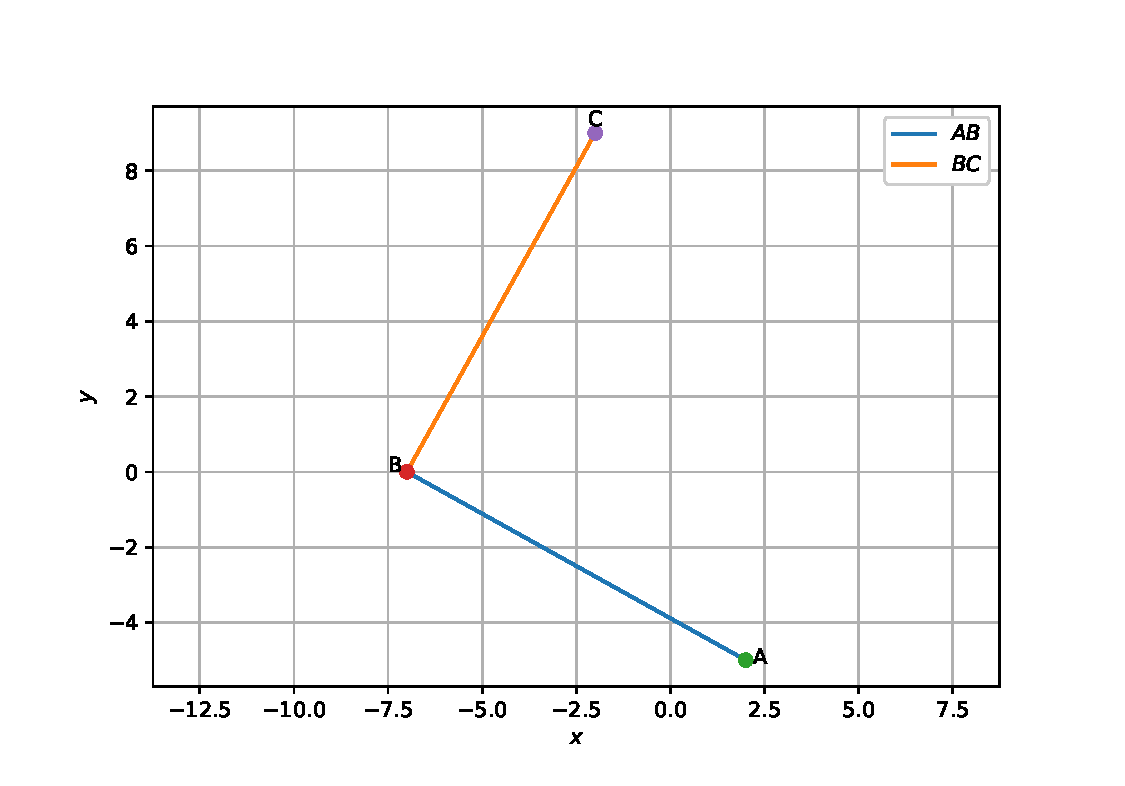
\includegraphics[width=\columnwidth]{./solutions/6/codes/line/point_vector/point_vector.eps}
\caption{}
\label{fig:3.5.6line_1}
\end{figure}

